\documentclass[psamsfonts,onesided,10pt]{amsart}
\usepackage{goodstyle}


%opening
\title{HW 3 - Write Up}
\author{Robin Belton, Daniel Laden, Jiahui Ma,  Badr Zerktouni}

\begin{document}

\maketitle

\section{System Usage}

This system was written with Python version 3.7 and uses Iris Data csv located at \path{https://github.com/jiahuiblair/CSCI-550/HW3/iris.csv} 
to test clustering and assessment algorithms. All python functions and packages are included in the \path{main.py} file.

All functions can be run in the command line as follows:

\begin{description}
\item[$k$-Nearest Neighbors] We describe how to provide classification labels to the testing dataset based on the $k$-nearest neighbors from the training dataset. The function is written for the Iris data. The user needs to specify how large the training dataset will be by indicating which attributes to use. To run the \textsc{$k$\_nearest} function, run \textsc{$k$\_nearest}(training\_data, labels, testing, $k$) where 
	\begin{itemize}
	\item training\_data is a dataframe with first four dimensions from Iris data including sepal length, sepal width, petal length and petal width from the training dataset.
	\item labels is is a dataframe only containing the species dimension in Iris data.
	\item testing is a dataframe with first four dimensions from Iris data including sepal length, sepal width, petal length and petal width from the testing dataset.
	\item $k$ is the number of nearest neighbors to used to classify a point.
	\end{itemize}. 
The output is a dataframe with both new labels and old labels of the testing data.
\item[Decision Tree] 
\item[$k$ Fold Cross Validation] 
\item[$F$-measure] To compute the $F$-measure of the clustered Iris data, run \textsc{Fmeasure}$(D)$ 
where $D$ is a six-dimensional dataframe with attributes: Sepal Length, Sepal Width, Petal Length, Petal Width,
              Species, and New Label, where the New Label is from the cluster identification. 
\end{description}
 
\section{Example of Input/Output}
\begin{description}
\item[$k$-Nearest Neighbors] This is an example of running the \textsc{$k$\_nearest} function
\begin{verbatim}
k_nearest(training_data,labels,testing,4)
\end{verbatim}
	\begin{figure}[H]
    	\centering
    	{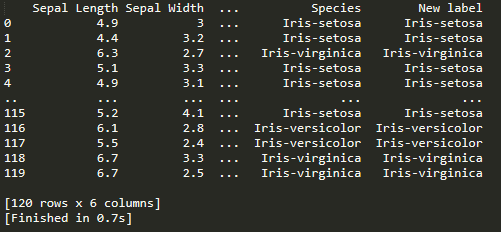
\includegraphics[width=.4\textwidth]{images/knearest.PNG}} 
   	 \caption{$k$\_nearest neighbors output dataframe}
	\end{figure}
	

\item[Decision Tree] \todo{}

\item[$k$ Fold Cross Validation] \todo{}

\item[$F$-measure] Below we take the output from $k$-nearest neighbors when $k=4$ and then compute the $F$-measure. 
\begin{verbatim}
D = k_nearest(training_data,labels,testing,4)
Fmeasure(D)
# output = 0.9544753086419752
\end{verbatim}
\end{description}

\section{Exploring Datasets}
In this section we describe our findings from Part 4. We explored how varying $k$ affected the 
output of $k$-nearest neighbors, how applying the clustering algorithms on lower dimensional 
subsets of the data affected the output, and compared $k$-nearest neighbors to the decision 
tree on the Iris dataset. 

First, we varied $k$ to see how this parameter affected the output of $k$-nearest neighbors on 
the Iris dataset. For this particular dataset, we found that even setting $k$ to as low as one gave 
a high $F$-measure. For $k\in \{1,...,15\}$, we got a $F$-measure above 0.9. However, 
once $k>15$, then the $F$-measure dropped significantly and in some cases was not even 
defined since not many points were being classifed as Iris-setosa. Overall, we were happy with 
how $k$-nearest neighbors performed in classifying the Iris species. Below is a plot of the true 
classification and the $k$-nearest neighbors classification for $k=4$. 

\begin{figure}[H]
    \centering
    {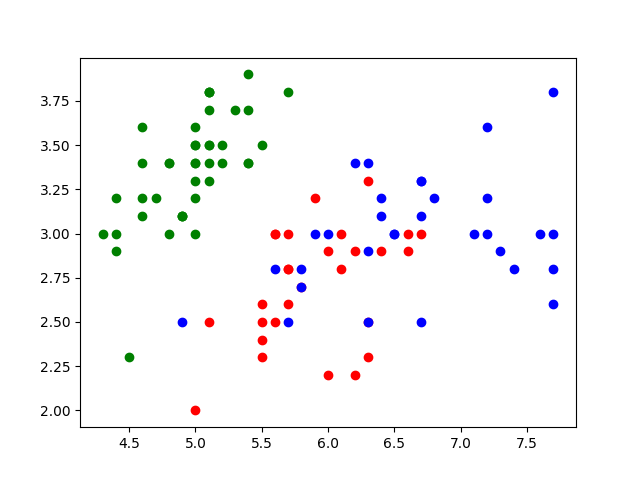
\includegraphics[width=.4\textwidth]{images/trueclass.png}} 
    {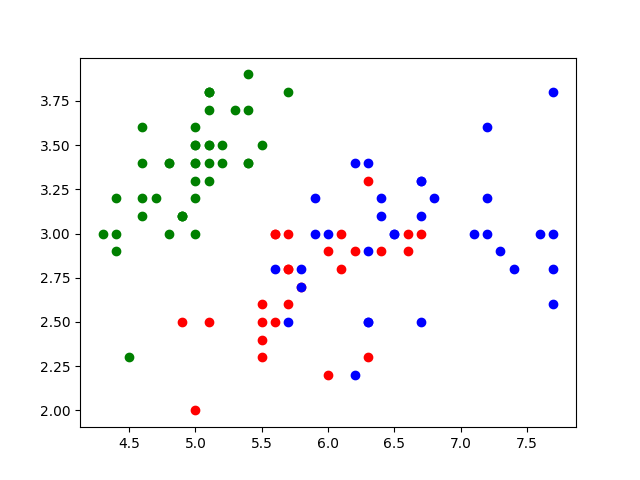
\includegraphics[width=.4\textwidth]{images/KNNclass.png}} 
    \caption{Plots of Sepal Length vs. Sepal Width of the Iris dataset. Left. The true classification 
of species is indicated by color. Right. Classification of species by $k$-nearest neighbors when 
$k=4$ is indicated by color. For both plots Versicolor is red, Virginica is blue, and Setosa is green.}
\end{figure}

We also applied $k$-nearest neighbors $(k=4)$ on lower dimensional subsets of the Iris dataset 
and computed the $F$-measure. See Table 1. We found that as we increased the dimension of 
our data to classify Iris species, the performance of the classification became better. 

\vspace{1ex}
\begin{center}
\begin{tabular}{ |c|c|c| } 
 \hline
\textbf{Attributes used for Classification} & \textbf{$F$-measure} \\ 
\text{SL} & 0.53 \\ 
\text{SL, SW} & 0.65 \\ 
\text{SL, SW, PL}  & 0.95\\
\text{SL, SW, PL, PW} & 0.95\\
 \hline
\end{tabular}\\
\textbf{Table 1.} $F$-measure assesments assessments applied to $k$-nearest neighbors classification.  
Attributes used for classification include: Sepal Length (SL), Sepal Width (SW), Petal Length (PL), Petal Width (PW).
\end{center}
\vspace{1ex}

In addition to the results in Table 1, we found that the Petal Length attribute was good for 
classifying. When we just used the Petal Length attribute for classification in $k$-nearest neighbors, 
we computed an $F$-measure of $0.94$. 

\end{document}
